The previous chapter addressed different aspects of a cooperative perception system conceptually. First, a uniform, expressive and extensible way to model traffic scenes for cooperative perception was proposed alongside an appropriate representation format for it. Different characteristics and benefits of 5G cellular networks were discussed before a high-level system architecture, involving a multitude of different modular software components was elaborated. Eventually, a concept was presented on how to combine observations from different actors, while taking temporal delay and uncertainty into account. 
\par
\bigskip
 
The purpose of this chapter is to pick up the previously presented concepts and techniques and explain how they were implemented in software. This includes a discussion about various technological choices, the use of appropriate software design patterns and essential performance-related considerations.
\par
\bigskip

During the implementation process, design- and component principles presented in \cite{Martin2017} were followed with the purpose to develop clean, modular and maintainable software components.

\section{Meta Model, Representation- \& Message Format}
\label{sec:implementation:meta_model_representation_message_format}

\subsection{Object-Oriented Model}
\label{subsec:implementation:object_oriented_model}
The meta model presented in \autoref{sec:concept_design:environment_modeling_state_representation} to be used to capture traffic scenes is a Probabilistic Entity Relationship Model, i.e. essentially an ER model, that is extended to incorporate a notion of structural- and relational uncertainty. As explained earlier, it can be viewed as a graph in which entities relate to other entities or attributes with a certain probability or confidence. Accordingly, the graph can also be represented as a collection of quadruples $r_i = \langle \textit{subject}, \textit{predicate}, \textit{object}, \textit{confidence} \rangle$, or, more formally $r_i \in \{ \langle \mathcal{E} \times \mathcal{A} \cup \mathcal{R} \times \mathcal{E} \cup \mathcal{L} \times \Gamma \rangle \}$. 

In code, this graphical structure is implemented as a composition of pure object-oriented classes. As Python was chosen as the primary programming language, the built-in Python class system is employed. Each type of entity corresponds to a certain class, which inherits from an abstract \textit{Entity} class. Relations (both entity-entity and entity-attribute) relations are implemented as sub-classes of an abstract \textit{Relation} class, which is attached to its object as a class member and holds members for its object (either a literal attribute or another entity) and the corresponding confidence. Deviating from the quadruple structure, an exception is introduced for convenience to additionally allow for the specification of attributes without uncertainty as well. Such are simply implemented as ordinary class members and should only be used to encode meta data, but not actual observations. Listing \ref{lst:class_example} depicts a simplified example of this modeling schema.

Most of the entities, attributes and relations from the final model, presented in \autoref{subsec:concept_design:the_final_model}, were implemented according to the above class schema and encapsulated as a re-usable Python library.

\inputminted[fontsize=\footnotesize]{python}{97_listings/class_example.py}
\captionof{listing}{Example Implementation of PER Entities and Relations}
\label{lst:class_example}

\subsection{Serialization Format}
\label{subsec:implementation:serialization_format}
The object-oriented schema presented in the previous section is used as a module throughout all related Python code. However, instances of these classes only exist within the scope of a certain process. In order to transfer these information across different program, which are potentially even written in different programming languages, a language-agnostic, commonly understandable format is needed. In technical terms, objects must be \textit{serialized}, then transmitted and \textit{deserialized} again afterwards. Multiple common serialization formats exists, which differ with respect to certain properties. Some are text-based and potentially also human-readable, others are binary formats and only understandable by machines. While text-based formats are generally more common and easier to work with, \autoref{subsec:concept_design:messaging_further_considerations} motivated the use of binary formats for performance- and efficiency-critical applications like CP.

Common binary serialization formats include Apache Thrift\footnote{\url{https://thrift.apache.org/}}, Cap'n'Proto\footnote{\url{https://capnproto.org/}},  Flatbuffers\footnote{\url{https://google.github.io/flatbuffers/}} and Protocol Buffers\footnote{\url{https://developers.google.com/protocol-buffers/}} (Protobuf). Most of them follow the principle of first defining a static class (or message) schema, which is then compiled to language-specific code to be used by different applications equally. During the serialization, objects and attributes are condensed to a highly efficient binary representation, which can usually be accessed as a byte stream or -array subsequently. Since all of these format are relatively similar, a detailed comparison and evaluation is out of scope.

In a first iteration \textbf{Cap'n'Proto} was used in the context of this work. Reasons for this decision included the high serialization performance claimed on the authors' website and the framework's novelty. However, as this work progressed, it became clear that serialization was a major performance bottleneck. In search of alternatives to Cap'n'Proto a brief evaluation\footnote{\url{https://github.com/n1try/talkycars-thesis/tree/master/src/evaluation/serialization}} revealed superior performance of \textbf{Protocol Buffers} format in comparison. In a simplified example, Protobuf was able to serialize \SI{7490}{messages\per\second} on average, compared to \SI{4129}{messages\per\second} with Cap'n'Proto (see \autoref{sec:appendix:evaluation_results:serialization_benchmark}). Moreover, the average message size with Protobuf appeared to be up to $\sim$ 47 \% smaller for the same payload. The benchmarking was done using the Go programming language, Google's reference implementation of Protobuf for Go and the most common third-party open-source Go implementation of Cap'n'Proto\footnote{\url{https://github.com/capnproto/go-capnproto2}}. 

The performance improvement of $\sim$ 25 \% and potential size decrease of up to 47 \% led to the decision to refactor existing code and use Protocol Buffers for serialization over the course of this work.

Listing \ref{lst:serialization_schema_examples} gives an example for a simplified message schema definition in Protobuf and Cap'n'Proto, respectively.

\begin{figure}[!h]
	\begin{minipage}{0.5\textwidth}
		\centering
		\inputminted[fontsize=\footnotesize]{text}{97_listings/protobuf_snippet.proto}
	\end{minipage}
	\begin{minipage}{0.5\textwidth}
		\centering
		\inputminted[fontsize=\footnotesize]{text}{97_listings/capnp_snippet.capnp}
	\end{minipage}
	\captionof{listing}{Exemplary schema definitions in Protocol Buffers (left) and Cap'n'Proto (right)}
	\label{lst:serialization_schema_examples}
\end{figure}

\section{Simulation Environment}
\label{sec:implementation:simulation_environment}
Since the integration and evaluation with an autonomous driving simulator is one of the core goals of this thesis, an appropriate simulator needs to be chosen. A commonly used option is \textbf{SUMO}\footnote{\url{https://sumo.dlr.de/}} (Simulation of Urban Mobility). However, it focuses on traffic simulation and it not particularly built for in-depth simulations of autonomous driving. Instead, a variety of high-detail, photorealistic 3D simulators have established recently. The most commonly used options are the following.

\begin{itemize}
	\item \textbf{AirSim} by Microsoft \cite{airsim2017fsr} is an open-source ($\sim$ 9,300 GitHub stars) 3D simulator for autonomous cars and drones based on the Unreal 4 game engine\footnote{\url{https://www.unrealengine.com}}. It has inherent support for Reinforcement Learning, allows to connect various kinds of external control devices and has a rich C++ and Python API to program it. Supported sensors are RGB camera, IMU, GPS, magnetometer, barometer, a custom distance sensor and LiDAR. 
	\item \textbf{Carla} \cite{Dosovitskiy17} is an independent open-source project (3,600 GitHub stars). The 3D simulator is based on Unreal 4, has C++ and Python APIs and features a multitude of sensors, including RGB camera, depth camera, IMU, GPS and LiDAR. In addition, is has multi-agent support, i.e. allows multiple Python- or C++ clients to connect to the simulation server and offers an integration with the Autoware AV stack\footnote{\url{https://www.autoware.ai/}}.
	\item \textbf{Carmaker}\footnote{\url{https://ipg-automotive.com/de/produkte-services/simulation-software/carmaker/}} by IPG Automotive GmbH is a proprietary 3D simulator featuring various integrations with hardware platforms and tools and offers an proprietary and a MATLAB programming interface.
	\item \textbf{LGSVL}\footnote{\url{https://www.lgsvlsimulator.com}} by LG is the latest of these 3D simulator projects, as development started in 2019. It is open-source ($\sim$ 700 GitHub stars), written in C\# and based on the Unity game engine\footnote{\url{https://unity3d.com}}, offers integrations with Autoware and Baidu's Apollo framework\footnote{\url{https://github.com/ApolloAuto/apollo}} and a Python API. Supported sensors include RGB camera, IMU, GPS, LiDAR, radar and CAN bus. While this project appears to be the most ambitious and promising one, it is still in quite early development and therefore partially unstable.
\end{itemize}

\begin{figure}[h]
	\centering
	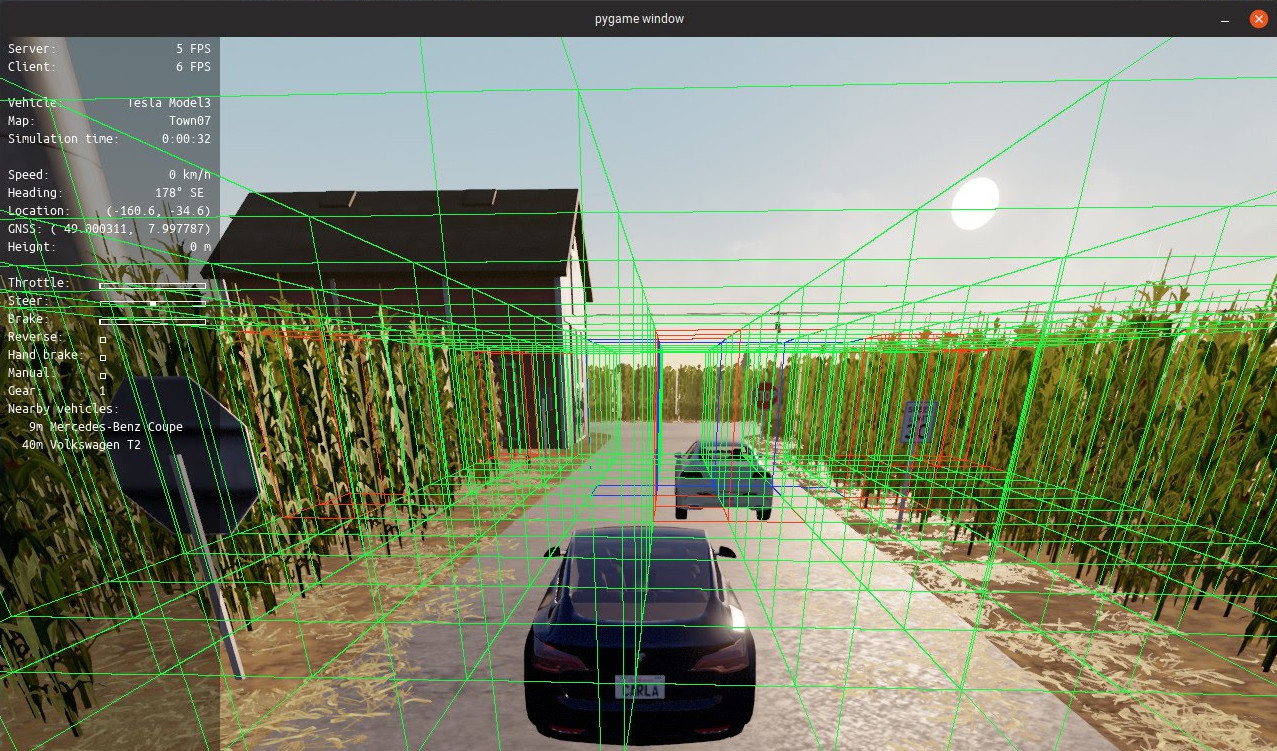
\includegraphics[width=0.9\linewidth]{98_images/carla_screenshot_1}
	\caption[Screenshot of an Exemplary Carla Scene]{Screenshot of an Exemplary Scene in Carla featuring two Vehicles and their Occupancy Grids}
	\label{fig:carla_sceenshot_1}
\end{figure}

Mainly because of its extraordinarily rich and intuitive API, the large number of simulated sensors and the inherent multi-agent support, Carla was chosen to be used as a simulation environment in this work. In addition to the features mentioned above, it also includes seven pre-defined high-detail maps, each of which represents a different scenario (e.g. urban or rural environments). Maps can be exported in the OpenDrive format and thanks to an integration with the RoadRunner\footnote{\url{https://www.vectorzero.io/}} software suite, custom maps can be created and imported easily. In addition to vehicles, pedestrians and cyclists are supported as traffic participants as well and the open-source community has provided automated controllers and navigation script for each of these actor types.

The screenshot in \autoref{fig:carla_sceenshot_1} depicts an exemplary rural scene in Carla, involving two vehicles. It was recorded at development stage when the simulation client already supported to compute and render the occupancy grid corresponding to an ego vehicle's observations. Green cells are considered free, red cells are occupied and the state of blue cells is unknown, e.g. due to sensor noise or because they are out of sight.